\documentclass{article}
\usepackage[utf8]{inputenc}
\usepackage{amsmath, amssymb, amsthm, cancel}
\usepackage[shortlabels]{enumitem}
\usepackage{caption}
\usepackage{graphicx}
\usepackage[top=1in, bottom=1in, left=1in, right=1in]{geometry}
\usepackage{float}

\title{\textbf{CSCI4150U: Data Mining}\\Lab 03 - Model Selection and Evaluation}
\author{Syed Naqvi \\ Student ID: 100590852}
\date{\today}

\begin{document}

\maketitle

\begin{abstract}
This report walks through the preprocessing steps, model selection, and evaluation methods used for Naive Bayes,
k-Nearest Neighbors, and Decision Tree classifiers to improve accuracy for a dating site recommendation system.
Models are trained using a training dataset with the final model selection based on performance metrics evaluated
using an unseen test dataset.
\end{abstract}

\section{Introduction}
In this experiment, we apply standard data preprocessing techniques, explore feature relationships, and select optimal models for classification using Naive Bayes, k-Nearest Neighbors (K-NN), and Decision Tree algorithms. Each model is evaluated using cross-validation, and the best models are selected based on accuracy and generalizability.

\section{Preprocessing and Exploration}
Data preprocessing involves standardizing features to ensure they have a mean of zero and a standard deviation of one, enhancing model performance. We visualize the distribution of standardized features and inspect feature pair correlations.

\begin{figure}[H]
    \centering
    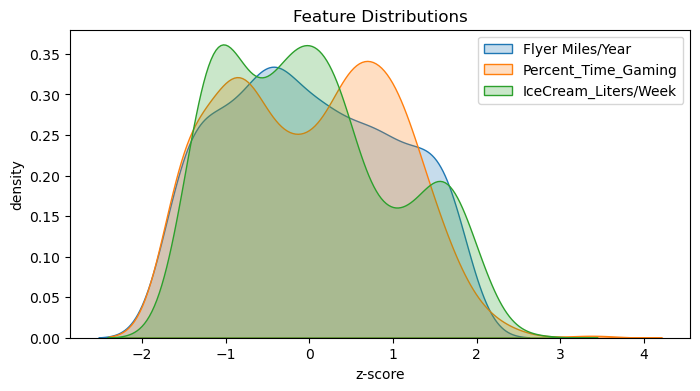
\includegraphics[width=0.8\textwidth]{pre_a.png}
    \caption{Distribution of Standardized Features}
    \label{fig:standardized-distribution}
\end{figure}

\begin{figure}[H]
    \centering
    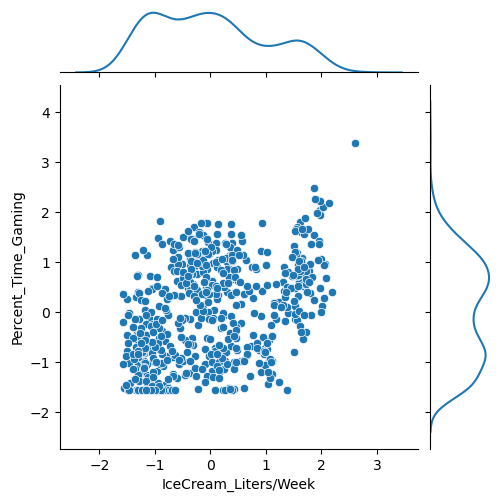
\includegraphics[width=0.47\textwidth]{pre_b.png}
    \caption{Percentage Time Gaming vs Ice Cream Liters/Week}
\end{figure}

\begin{figure}[H]
    \centering
    \begin{minipage}[b]{0.47\textwidth}
        \centering
        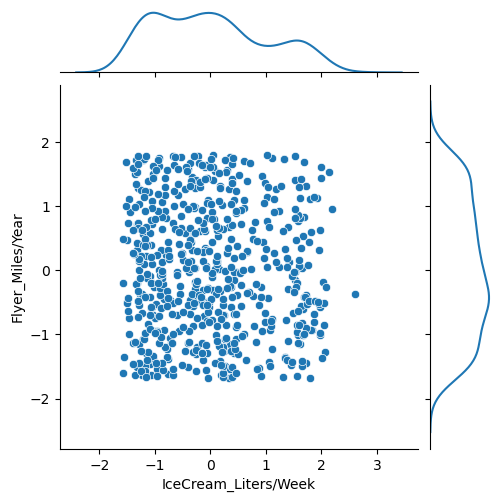
\includegraphics[width=\textwidth]{pre_c.png}
        \caption{Flyer Miles/Year vs Ice Cream Liters/Week}
    \end{minipage}
    \hfill
    \begin{minipage}[b]{0.47\textwidth}
        \centering
        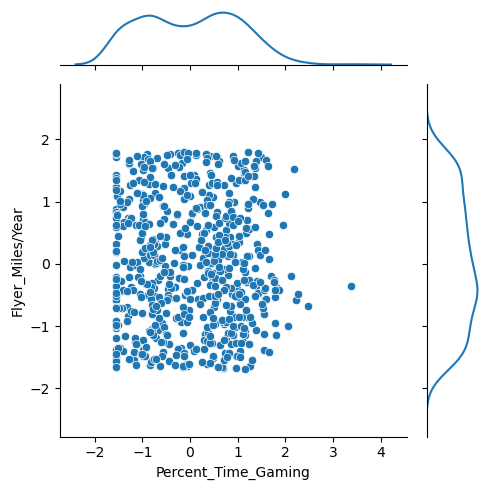
\includegraphics[width=\textwidth]{pre_d.png}
        \caption{Flyer Miles/Year vs Ice Cream Liters/Week}
    \end{minipage}
\end{figure}

\newpage

\section{Naive Bayes Classification (Gaussian Distribution)}
\subsection{Model Validation}
Naive Bayes is selected due to minimal correlation between features, suggesting a high degree of independence. The cross-validation results for the Gaussian Naive Bayes model are presented in Figure~\ref{fig:nb-results}.

\begin{figure}[H]
    \centering
    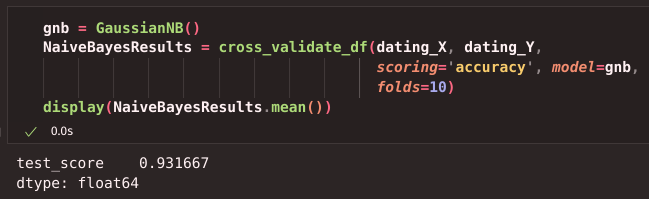
\includegraphics[width=0.75\textwidth]{NB_results.png}
    \caption{Naive Bayes Cross Validation Results}
    \label{fig:nb-results}
\end{figure}

\section{K-Nearest Neighbors (K-NN) Classification}
\subsection{Model Selection}
To determine the optimal $k$ value, we evaluate k values in the range $[1,30]$ using 10-fold cross-validation. The average accuracy per k-value across 100 iterations is recorded, with $k=18$ yielding the highest accuracy.

\begin{figure}[H]
    \centering
    \begin{minipage}[b]{0.49\textwidth}
        \centering
        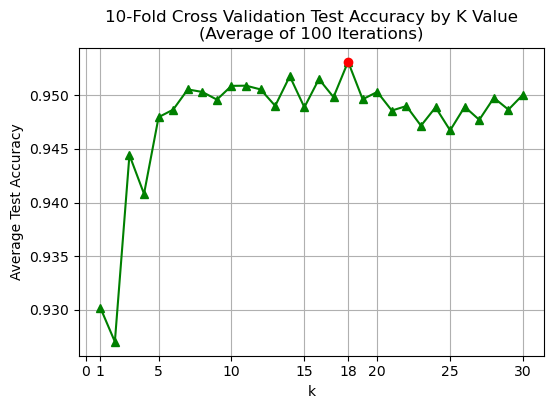
\includegraphics[width=\textwidth]{k-NN_selection.png}
        \caption{Accuracy vs. K for K-NN}
    \end{minipage}
    \hfill
    \begin{minipage}[b]{0.49\textwidth}
        \centering
        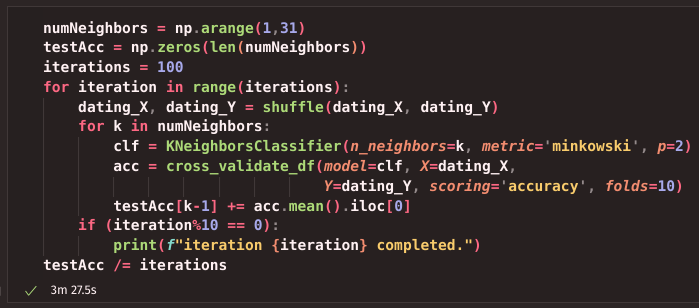
\includegraphics[width=\textwidth]{k-NN_selection_code.png}
        \caption{Code for Best K Selection}
    \end{minipage}
\end{figure}

\newpage

\section{Decision Tree Classification}
\subsection{Model Selection}
We create decision trees with varying depths, using entropy and Gini impurity measures, and apply 10-fold cross-validation to identify the depth and impurity measure yielding the highest accuracy.

\begin{figure}[H]
    \centering
    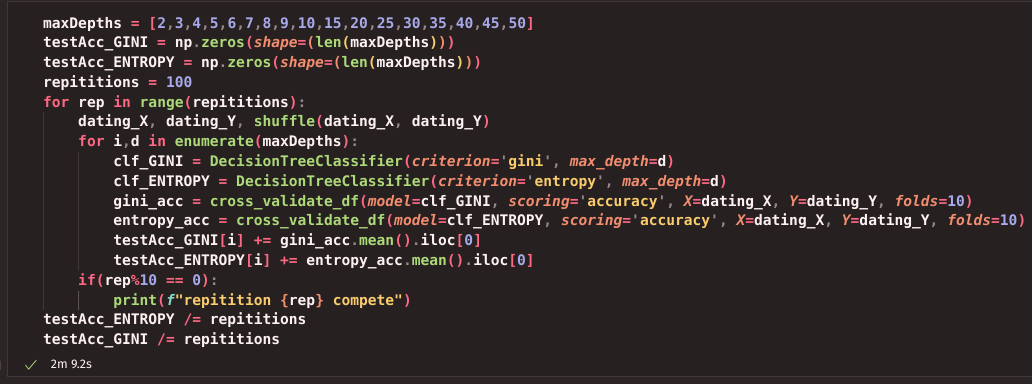
\includegraphics[width=0.7\textwidth]{tree_selection_code.png}
    \caption{Decision Tree Model Selection Code}
\end{figure}

\begin{figure}[H]
    \centering
    \begin{minipage}[b]{0.49\textwidth}
        \centering
        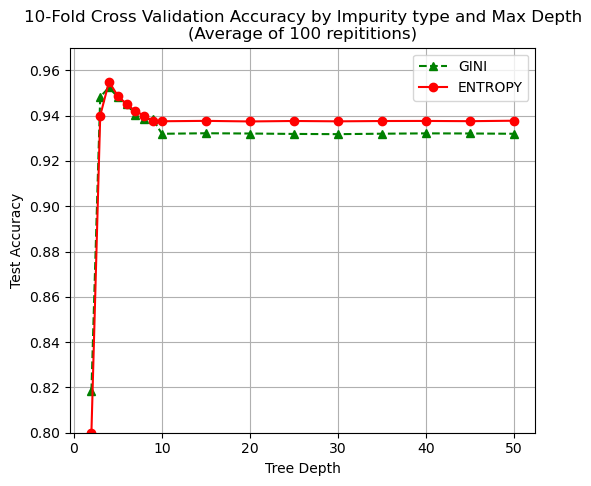
\includegraphics[width=\textwidth]{tree_selection1.png}
        \caption{Accuracy by Impurity and Depth}
    \end{minipage}
    \hfill
    \begin{minipage}[b]{0.49\textwidth}
        \centering
        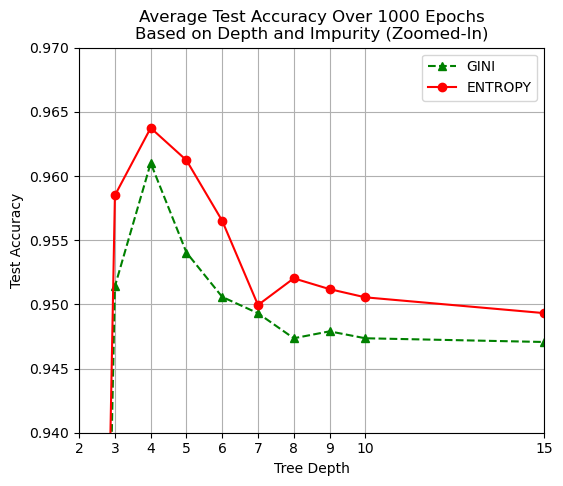
\includegraphics[width=\textwidth]{tree_selection2.png}
        \caption{Zoomed-In Accuracy by Impurity and Depth}
    \end{minipage}
\end{figure}

The optimal decision tree model uses entropy impurity with a maximum depth of 4.

\newpage

\section{Test Set Validation}
After model selection, we evaluate the chosen models on the test dataset. The comparison results are shown in Figure~\ref{fig:model-comparison}.

\begin{figure}[H]
    \centering
    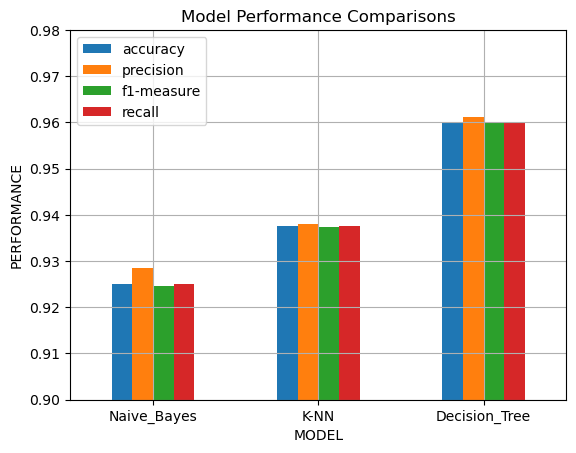
\includegraphics[width=0.7\textwidth]{comparison.png}
    \caption{Comparison of Model Performance}
    \label{fig:model-comparison}
\end{figure}

\begin{figure}[H]
    \centering
    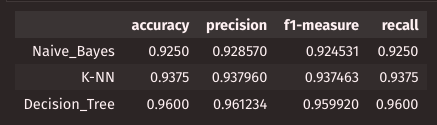
\includegraphics[width=0.7\textwidth]{comparison_table.png}
    \caption{Model Performance Summary}
\end{figure}

\section{Conclusion}
Based on the test dataset results, the decision tree model with entropy impurity and a max depth of 4 demonstrates the
best classification performance. This model is recommended for predicting customer dating preference based on provided
features.

\end{document}
